\chapter{Event reconstruction and simulation}
\label{ch:simreco}
The basic quantity for readout, reconstruction, and further processing as well as data analysis is called the `Event' and refers to a full readout of the
CMS detector. This chapter explains the various steps leading from an actual physical bunch crossing with proton-proton collisions taking place within CMS 
to a reconstructed event which can be used for data analysis. First, a sequence of data reduction has to take place in order to cope with the stupendous amount
of data produced by the CMS detector. Secondly, the binary data coming out of the electronics has to be combined into a physical picture of a collision or an event
using specifically designed software frameworks and reconstruction code. Lastly, this chapter also gives a short overview on how physics processes can be simulated
and how this can be combined with a simulated version of the CMS detector for the production of background and signal data samples which are then used for
the ensuing data analysis.


\section{The trigger system}
\label{sub:cms_trigger}
With a bunch crossing frequency of \SI{40}{\mega\hertz} and a mean number of collisions per bunch crossing of roughly 20, there are of the order of 800 million collisions taking
place inside CMS every second. Considering that the whole of CMS has roughly 100 million readout channels, this would lead to unsustainable data-rates, even for the most 
powerful readout and network possible to date. For this reason, a triggering system has been implemented in order to differentiate `interesting' collisions from those
who are considered not. CMS has adopted a two-stage approach, with a first, hardware-based and thus very fast triggering mechanism called the Level-1 trigger (L1), followed
by a second, fully software based trigger named the High-Level-Trigger (HLT). 

\subsection{The L1 trigger}
\label{sub:l1}
Dealing with complicated data at a rate of \SI{40}{\mega\hertz} requires for processing of information at speeds that are unattainable for software reconstruction. 
Therefore, a fully hardware based system has been implemented, relying heavily on the use of integrated circuits in the form of so-called Field-Programmable-Gate-Arrays (FPGAs).
Because speed is such an important point of the triggering decision, not all information from the detector can be used in order to make a yes/no decision on an event-by-event
basis. In the current L1 trigger system, only coarsely segmented information from the calorimeters and the muon system are used for the trigger decision, 
while the full data from the muon system, the calorimeter, and the silicon tracker are stored in buffers until a trigger accept (L1 accept) triggers the full readout of these buffers.
An organizational sketch of the different participants for a trigger decision is shown in Fig.~\ref{fig:l1}
\begin{figure}[h!]
    \centering
    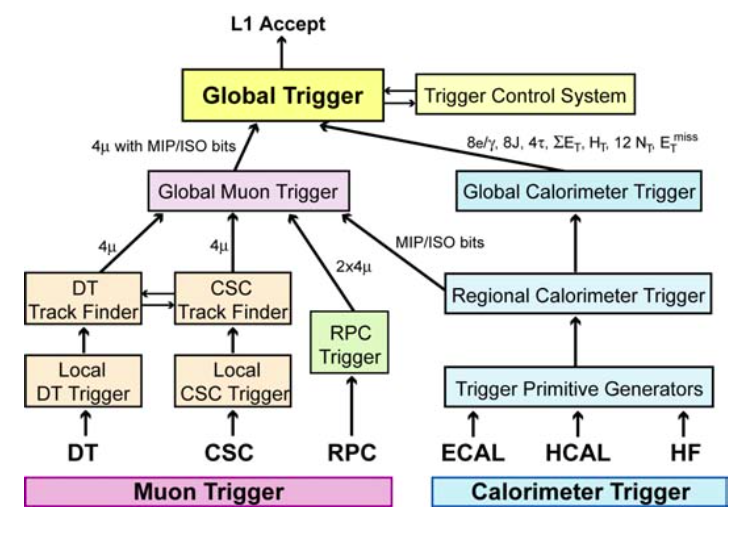
\includegraphics[width=0.65\textwidth]{../figs/l1_organi.png}
    \caption{Organizational chart of the various components of any L1-accept. The two systems (calorimetry and muons) work in parallel 
until they are combined at a regional/global level into the global trigger decision~\cite{cmsdetector}.}
    \label{fig:l1}
\end{figure}
The calorimeter part of the trigger has inputs from the ECAL, HCAL, and the HF, constructing first so-called Trigger Primitives from coarsely organized trigger `towers'. These are
then fed into a regional trigger, where energy sums and crude identifications of physical objects are performed. This information is then given to the global trigger, which constructs
relevant variables such as the total energy deposited, the number of jets, etc.
In parallel, the muon system tries to identify tracks of muons and calculate their \pt by taking information from all three sub-systems and combining it into the Global
Muon trigger. This output is then combined with the calorimeter trigger into a final trigger decision, the aforementioned L1-accept.


The input rate to the L1 is the bunch crossing frequency of the LHC and the maximum processing time of the L1 logic is \SI{3.2}{\micro\second}. The output rate, 
i.e. the rate of L1-accepts, is limited to \SI{100}{\kilo\hertz}. At this rate, the
L1-accept is passed to all the subdetectors, triggering full readout of the event information stored in buffers. This set of complete data is then passed on to the HLT.

\subsection{The HLT}
\label{sub:hlt}
At the L1 output rate, the full information from the detector is sent from the experimental cavern at P5 to a computer farm situated above ground for further processing.
This computer farm is made of a large number of commercial CPUs (in total about \num{13000}) cores, running reconstruction software which is implemented into the whole 
CMS reconstruction software, package 
described below in section~\ref{sub:cms_reco}, albeit with different sets of parameters optimized for speed~\cite{hltcms, hltcms2}. The HLT starts with L1 information on the candidates for
physical objects, and improves the reconstruction. The organization is done in so-called HLT paths, which are essentially requirements on physical objects being present in
a collision. An example which will be used later on in the analysis part of this thesis is \texttt{HLT\_Mu17\_Mu8\_v1}, which requires the presence of one muon with \pt
greater than 17 \gev and another muon with \pt greater than 8 \gev on HLT level. Other `online' physical objects in the HLT include electrons, jets, missing transverse
energy, and \HT -- the scalar sum of all jet-$p_T$s above a threshold. The reconstruction of objects is divided into modules for any given quantity, followed by a filter on 
the quantity where a cut is applied, in order to save precious computation time of unnecessary quantities. The largest fraction of computation time is taken up by the tracking, and
the total time required for an event depends on the exact event kinematics, up to a limit of \SI{200}{\milli\second}.

The total data reduction factor of the HLT system is roughly \num{10e2}, so the final output rate of events actually fully reconstructed and saved on hard-drives is of the order
of \SI{1}{\kilo\hertz}. About half of this data is reconstructed in the immediate time period after the collision, whereas the other half of the data is first stored and 
reconstructed only later, when computing resources for reconstruction are freed. This process is called data-parking and was implemented for the first time in 2012.

To facilitate analysis of the data when it is fully reconstructed after passing the HLT, different HLT paths are organized in various so-called primary datasets (PDs), which group similar
events into one collection. Examples for primary datasets are DoubleMu, DoubleElectron, and MuEG.

\section{Reconstruction and data formats}
\label{sec:cms_reco}
Upon passing the HLT at P5, collision data are sent to the CERN Tier-0 computing center located at the CERN main site in Meyrin for full reconstruction at a rate of roughly \SI{1}{\kilo\hertz}. 
Full reconstruction of each triggered event is then performed by the CMS software framework called CMSSW (FIXME cite). For data analysis it is necessary
to obtain a data format in which physical objects can be identified, this is called the \textit{Event Data Model}, EDM. CMSSW reconstructs different detector related quantities
such as calorimeter energy deposits, tracks from the pixel and strip tracker and muons from the muon chambers, with the best available precision and places those objects into the EDM. 
It also combines those quantities into physical particles and observables as described below.

Tracks are reconstructed using an iterative tracking algorithm where in a first iteration tight criteria for track-seeding are used in order to minimize reconstruction of
fake tracks. In subsequent iterations the set of previously found tracks are used as input, loosening the track fitting requirements to regain tracking efficiency. Five iterations
are done, leading to efficiencies of about 99.5\% for muons, and well above 90\% for charged hadrons within the tracker volume. Tracks with as little as three hits in the ~10 layer
tracker can be reconstructed, with a minimal transverse momentum of about 150 \mev, while the fake rate is kept to below one percent~\cite{pfcms}.

Calorimeter clusters are reconstructed by searching for calorimeter cells with an energy deposit above a certain seed-threshold. These are then combined with adjacent cells
beyond a threshold equivalent to about twice the electronic noise (80-300 \mev in the ECAL and 800 \mev in the HCAL).

Subsequently, these detector-based objects are combined through an algorithm called `Particle Flow' (PF) to identify candidates for physical objects.

\subsection{Particle flow}
\label{sub:pf}
The particle flow algorithm~\cite{cmspf} aims at reconstructing an integral picture of every triggered bunch crossing by combining information from all subdetectors to identify
PF candidates. These are photons, electrons, muons, neutral hadrons, and charged hadrons. 

First, tracks are combined with the information from the muon chambers 
to search for `global muons' which have both a track, and are reconstructed in the muon system. If a match is found, this PF muon is put into the appropriate collection in the EDM
and the track is removed from the collection of tracks. The second step involves the matching of tracks and energy clusters in the ECAL, producing a candidate electron. These are then
refit with a Gaussian Sum Filter (GSF) in order to account for bremsstrahlung on the electrons trajectory and the tracks are removed from the track collection. Remaining tracks are
then matched to HCAL deposits to construct a collection of charged hadrons. Any energy deposit that does not have an associated track, is then interpreted as a photon or a neutral
hadron, depending on the energy fractions in the ECAL and HCAL. 

The PF candidates obtained by this algorithm are then taken as the input to the clustering algorithm of hadronic jets. This jet clustering algorithm most widely used in CMS
is the so-called anti-$k_T$ clustering algorithm~\cite{antikt}, developed in 2008. This algorithm is both collinear, and infrared safe\footnote{Collinear safety describes invariance
of a jet's properties upon division of a constituent's energy into two collinear particles. Infrared safety refers to invariance of the jet upon addition of very soft, i.e. low-energetic,
particles} and the distance parameters of the clustering algorithm are

\begin{align}
    d_{ij} & = \text{min}\left( k_{T,i}^{-2}, k_{T,j}^{-2} \right) \frac{ (\Delta R)^2_{ij}}{R^2}, \\
    d_{iB} & = k_{T,i}^{-2}, \\
    d_{jB} & = k_{T,j}^{-2}.
\end{align}

In this equation, $R$ defines the radial size of a jet, $\Delta R$ is the spacial distance between two candidate particles $i$ and $j$, while $k_{T,i}$ and $k_{T,j}$ are the transverse
momenta of particles $i$ and $j$. If the minimum distance is either $d_{iB}$ or $d_{jB}$, the particle is called a jet and is removed from the collection. Whereas if the minimum distance
is $d_{ij}$, the two particles $i$ and $j$ are merged into a new particle. Because of the inverse exponent in the minimum of the two transverse momenta squared, this means that the 
anti-$k_T$ algorithm clusters soft particles around the hard particles before clustering of soft particles among each other takes place. This leads to perfectly circular jets (as long as
they do not overlap), facilitating corrections to be made due to pileup and other effects.

It is worthwhile to note here, that the PF algorithm in combination with the jet clustering produces overlaps between physical objects. As an example, a muon can enter both the muon
collection and can be reconstructed as a jet. It is therefore important to employ some cross-cleaning of objects in any analysis.

\subsection{Data formats}
Centrally reconstructed events are saved in various data formats all based on EDM, but with differing detail of content. The basic format is RAW, which stored the raw detector information. 
Output from the full reconstruction at the Tier-0 is saved in the RECO data format. This format allows for much flexibility, albeit at very large event sizes, rendering it impractical 
for daily use. The most used format for processing in data analyses is called AOD, Analysis Object Data. This is a simple subset of the RECO data format, containing all relevant information 
for data analysis. The event size of one RECO event is about 1.2 MB, while AOD events are of the order of 300 kB, depending on the kinematics of the event.

Each event is saved at least twice, one copy usually lying at the CERN Tier-0 computing center, and another copy distributed in the LHC Computing Grid (LCG), a worldwide network of computer 
centers for data analysis and storage. Analysis of the data is done with user-written programs running on AOD events. Since primary datasets are of significant size containing oftentimes
many million events at once, these programs are sent by the user via the LCG to a computing center which hosts the dataset of interest, rather than the dataset being copied to the user. The final
data formats used in small-scale analysis are ROOT based files~\cite{root}. ROOT is a data analysis framework conceived especially for data analysis at CERN. It features many convenient 
data formats, such as TTrees\footnote{See \texttt{http://root.cern.ch/root/html/TTree.html} for more details.}, and provides capabilities of producing plots, histograms, perform fits and many 
more functionalities.


\section{Simulation and Monte-Carlo}
\label{sec:cms_mc}
For a number of different reasons, it is necessary to be able to simulate physical processes from theoretical models such as the Standard Model or Supersymmetry and feeding them into
a simulation of the CMS detector.
These reasons include testing the behavior of the CMS detector, validation of known physical processes, background studies for searches for new physics, signal studies for physics searches
and many more. 
Complete simulation of a physics event in CMS is a very complicated and multi-layered process. It starts from the actual physical process from calculations with matrix elements, 
continues with the decay of the produced particles including hadronization of quarks and radiations during this process. Once a `stable' physical process is generated, the interaction
with the simulated version of the CMS detector has to be implemented in order to end up with a set of binary data similar to what comes out of regular data-taking. Once this step is 
achieved, the reconstruction software described in Section~\ref{sec:cms_reco} processes these data in the exact same way as collision events. This section gives a quick overview of 
all the steps involved and software packages capable of performing these different tasks.

\subsection{Simulation of hard parton scattering}
\label{sub:hard}
The underlying physical theories and mathematical framework of how to simulate and calculate scattering amplitudes was already described in section XX FIXME, however an implementation
of these complicated calculations will be discussed here. There are a number of tools on the market for this step of event simulation, which differ most notably in the order
of the perturbative expansion in the strong coupling constant, $\alpha_s$. They are all summarized as so-called Monte-Carlo (MC) generators, as they make heavy use of the Monte-Carlo method
of random sampling of distributions.

\subsubsection*{Parton distribution functions}
One important piece of input to calculate a hard parton scattering amplitude are the so-called parton distribution functions, PDFs. They describe at a given energy of the proton-proton
collision the probabilities of finding a given type of parton, gluons and (anti-)quarks, at a certain energy fraction $x$ of the proton. An example for PDFs from the MRST/MSTW collaboration
can be seen in Fig.~\ref{fig:pdfs}.  The red curve in Fig.~\ref{fig:pdfs} represents the gluon PDF, which is divided by a factor 10 in order to fit the scale, 
while the others are for quarks and anti-quarks. It is easy to see from these graphs, that overall parton-parton interactions at the LHC are dominated by relatively low-energy
gluon induced processes. Only processes which require a large invariant mass (i.e. large values of $x$ for both partons) are dominated by valence-quark induced processes. PDFs are measured
by performing fits to a wide range of kinematic distributions from collider experiments, especially from deep inelastic electron-proton scattering. Alongside
the commonly used MRST/MSTW PDF sets, there are others used within CMS such as CTEQ, and NNPDF~\cite{nnpdf,cteq}. 

\begin{figure}[h!]
    \centering
    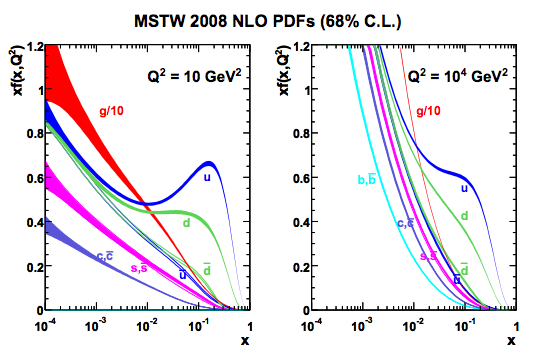
\includegraphics[width=0.65\textwidth]{../figs/pdfs.png}
    \caption{Parton distribution functions of the proton for two different resolution scales $Q^2$. This particular set of parton
    distribution functions is obtained from the MRST/MSTW collaborations~\cite{mstw}.}
    \label{fig:pdfs}
\end{figure}

\subsubsection*{Hard scattering generators}
As briefly stated before, there are many different implementations of calculating the matrix element (ME) part of a hard partonic scattering. The main difference being the order of
$\alpha_s$ in which this calculation is done. Since higher order calculations are generally expected to give a better description of the process, higher order matrix element
generators are considered more accurate. The most commonly used leading order (LO) matrix element generator is \texttt{MadGraph}\cite{madgraph}, it not only does the leading order
matrix element calculations, but also includes the real corrections of the next-to-leading order contribution, while the virtual corrections are unaccounted for. Most simulated
samples used in the data analysis section of this thesis use \texttt{MadGraph} in version FIXME. An example of a fully next-to-leading order (NLO) matrix element generator is 
\texttt{POWHEG} ~\cite{powheg}, capable of calculating MEs of most relevant processes at the LHC. Recently, the \texttt{MadGraph} ME generator has been combined with an NLO 
generator called \texttt{MC@NLO}~\cite{mcatnlo} into a common package called \texttt{MadGraph5\_aMC@NLO}\footnote{Creativity in name-finding was not given highest priority in the development
of this project.}, which will play a crucial role in future data analyses~\cite{madgraphamcatnlo}. In addition to the ME generators, there is a set of widely used multi-purpose event
generators that do not specifically calculate the matrix element, but rather use libraries of processes in order to simulate events. Examples for such more phenomenological event simulators
used at CMS are \texttt{PYTHIA} and \texttt{HERWIG}~\cite{pythia,herwig}. 
All the aforementioned generators do not only provide simulated events in the form of text-based files with the four-momenta of all the simulated particles, but they also give a
value for the cross-section of each process, which can then be used as a normalization to the data.

\subsection{Decays, hadronization, and radiations}
\label{sub:hadr}
After the generation of the hard scattering process, the produced particles have to be decayed in the case of non-stable particles, hadronized in the case of quarks in the final state, 
and appropriate radiations in both the initial-, and final state have to be added to the event. The decay of unstable particles is somewhat arbitrarily taken care of by the ME generator
for particles with a short lifetime, such as $W$ and $Z$ bosons, while longer living particles are usually decayed by the parton showering part described just below. There also exist a
few specific decay simulators in order to preserve proper spin-information in the decay of $\tau$ leptons and heavy resonances, named \texttt{Tauola} and \texttt{MadSpin}, 
respectively~\cite{tauola,madspin}.

Hadronization of quarks is done by the means of the multi-purpose MC generators mentioned before. Since the hadronization of quarks is an extremely challenging task to describe
in perturbative QCD (and outright impossible for bound states, for instance).


\subsection{Simulation of CMS}
\label{sub:geant}
